% ++++++++++++++++++++++++++++++++++++++++
% Don't modify this section unless you know what you're doing!
\documentclass[letterpaper,12pt]{article}
\usepackage{tabularx} % extra features for tabular environment
\usepackage{amsmath}  % improve math presentation
\usepackage{graphicx} % takes care of graphic including machinery
\usepackage[margin=0.75in,letterpaper]{geometry} % decreases margins
\usepackage{cite} % takes care of citations
\usepackage[final]{hyperref} % adds hyper links inside the generated pdf file
\usepackage{listings}
\usepackage{csvsimple}
\usepackage{verbatim}
\usepackage{float}
\usepackage{graphicx} % Allows including images
\hypersetup{
	colorlinks=true,       % false: boxed links; true: colored links
	linkcolor=black,        % color of internal links
	citecolor=blue,        % color of links to bibliography
	filecolor=magenta,     % color of file links
	urlcolor=blue         
}
%++++++++++++++++++++++++++++++++++++++++
\setlength{\parindent}{0pt}
\setlength\parskip{1em plus 0.1em minus 0.2em}

\begin{document}
\title{%
PyLab - Radioactive Decay \\
\large PHY224 Lab 2}
\author{Fredrik Dahl Bråten, Pankaj Patil}
\date{\today}
\maketitle
%\tableofcontents
%\listoffigures
%\listoftables

\section{Exercise 2:  Nonlinear fitting methods I}

\subsection{Abstract}

In this exercise, we measure and model the rates of emission over time from the radioactive decay of Barium (Ba-137m). 
We have chosen two models, one where the emission rate $I(t) = ae^{bt}$, and one where $\ln(I(t)) = at+b$, 
where $a$ and $b$ are parameters of each model to be fitted to our data, 
$t$ is time, and $ln$ is the natural logarithm. 
After fitting these models to our data, we graphically plot and 
compare these model curves along with the theoretical curve of emission rate, and our data with error bars. 
To evaluate the quality of our models, we calculate and discuss the $\chi^2_{red}$ values of our models and data, 
and confirm that the theoretically predicted half-life of Ba-137m lies within the estimated half life with 
uncertainty of our two models. 
This analysis was done in Python by use of the numpy, scipy and matplotlib modules.

\subsection{Introduction}

In this exercise, we measure and model the rates of emission over time caused 
by radioactive decay from a sample of Barium (Ba-137m). 
The corresponding theoretically predicted relationship between emission 
rate ($I$) and time ($t$) is:
$$I(t) = I_0e^{-t/\tau} = I_0 (\frac{1}{2})^{\frac{t}{t_{\frac{1}{2}}}}$$ 
Where $I_0$ is the initial emission rate, $\tau$ is the mean lifetime of the 
isotope, and $t_{\frac{1}{2}}$ is the half-life of the isotope. 
In our experiment, t is the independent variable, and I is our dependent variable.

We are modeling this relationship by using two models, one where the emission rate 
$I(t) = ae^{bt}$, and one where $\ln(I(t)) = at+b$, 
where $a$ and $b$ are parameters of each model to be fitted to our data, 
$t$ is time, and $\ln$ is the natural logarithm.

\subsection{Methods, Materials and Experimental Procedure}

We successfully followed the procedures as described in the exercise2-NL-fit.pdf \cite{lab-manual-ex2}
document.

The points of data for which we based this analysis on, 
was downloaded from Quercus as instructed by the TAs. 
The uncertainties of the measured data were calculated as described 
in the exercise2-NL-fit.pdf \cite{lab-manual-ex2} document.

\subsection{Results}

In Appendix Figure \ref{ba-count-rates} and \ref{ba-count-rates-log}, we see our data from the experiment 
plotted as points with corresponding error bars. 
Furthermore, we see the theoretical curve as described in the introduction, 
along with the curves corresponding to our two models best fitted to our data. 

The estimated optimal parameters with uncertainty by scipy optimize curve fit are: 

[a,b] = [-0.00393908  3.75408883] $\pm$ [0.00090733 0.29589009] for the linear model, and

[a,b] = [ 4.36112915e+01 -4.08767747e-03] $\pm$ [1.35411958e+01 1.00398911e-03] for the non linear model.

The $\chi^2_{red}$ values for the nonlinear and linear model, respectively, are 0.0069 and 0.0076.

The Half-life of the Barium, predicted by the non-linear model, is: 170.0 $\pm$ 42.0 seconds.

The Half-life of the Barium, predicted by the linear model, is: 176.0 $\pm$ 41.0 seconds.

\subsection{Discussion}

The $\chi^2_{red}$ values we found were very low. This means that our models 
fit our data very well. Thus, the Euclidian distance between the data points and 
our curves is in general very low. However, this is not necessarily a good sign. 
Our $\chi^2_{red}$ values should ideally both be equal to one. 
That we have extremely low $\chi^2_{red}$ values implies that we do not 
have enough data. It means that we are in risk of overfitting our models to our data.

The non-linear regression method gave a half-life closer to the expected 
half-life of 2.6 minutes = 156 seconds. 170 seconds is closer to 156 seconds, 
than 176 seconds, see half-life results in the Results section. Do however note 
that the theoretical half life falls within both of our models’ estimates of 
the half-lives, with associated uncertainties.

Though it is hard to distinguish the two models in the non-linear plot, in the 
logarithmic, linear plot, you can more easily see that the non-linear model 
returns a curve closer to the theoretical curve than the curve returned by the 
linear model. Both models do however fit the theoretical curve quite well. 
Furthermore, both models are well within the uncertainties of our measurements, 
see Figure 1 and 2 in the Results section.

\subsection{Conclusions}

In this exercise we estimated the emission rate caused by radioactive 
decay of Barium (Ba-137m). We successfully followed the instructions for 
the experiment written in the exercise2.pdf document without issues. 
Though both of our models of emission rate over time returned quite similar 
curves, the non-linear model returned a curve closest to the theoretical curve. 
We have plotted our data with error bars, our models, and the theoretical 
curve in a normal plot, and a plot with logarithmic y-axis. Furthermore, 
we have calculated and discussed each models $\chi^2_{red}$ value, 
and confirmed that the theoretical half-life of Ba-137m lies within each of 
our models’ predicted half-lives with uncertainties. 

\pagebreak

\section{Exercise 5:  Random number analysis}

\subsection{Abstract}
The aim of this exercise is to analyze the random radioactive decay in Fiesta dinner plates, which 
contain low amount of Uranium Oxide. The emissions from Fiesta plates are random and the data for 
the rate of emission can be recorded using Geiger counter. The analysis on this data is done using
the Python modules numpy, scipy and matplotlib. After the analysis, we concluded that the data 
collected for Fiesta plates obeys the rare event statistics given by Poisson distribution. We will discuss
the analysis of the data using the python data analysis modules in this report.

\subsection{Introduction}

Poisson Distribution is a \textbf{discrete probability distribution} that expresses probability of a given number 
of events in fixed interval of time if the events are known to occur with constant mean rate \cite{lab-manual-ex5}.
The Poisson \emph{probability mass function} is given by
$$P_{\mu}(n) = e^{-\mu}\frac{\mu^n}{\Gamma(n+1)}$$
Where $\mu$ is the expected average counts in measured counting interval and $\Gamma(n+1)$ is Gamma function. 

In this exercise, we analysis the radioactive counts from Fiesta dinner plates which contain Uranium Oxide in the glaze.
We followed the commonly followed approach in Radioactive decay experiments, of using histograms to analyze the counts data.

For the Fiesta plates the mean count, $\mu$, was found to be 126, and the same for background counts was 2.

\subsection{Methods, Materials and Experimental Procedure}

We successfully followed the procedures as described in the exercise5.pdf \cite{lab-manual-ex5}
document. The data was downloaded from Quercus for analysis.

\subsection{Results}

The data collected from Geiger counter was used to plot the histogram for the emission count. 
Figure \ref{fiesta-plate} shows the histogram for data collected along with the qualitative
fit of Poisson probability mass function. The histogram is plotted in normalized mode by setting $density=True$.
Gaussian distribution is also added to the same plot.

The measured count for Fiesta plate is corrected by subtracting the mean background emission counts. Figure \ref{fiesta-plate} shows the analysis done for Fiesta plates counts.

The expected average number of counts for Fiesta plate, per counting interval of 20 seconds, was found to be
$$\mu=126\text{\ \ \ \ with \ \ \ } \sigma = \sqrt{\mu} = 11.23$$
We note that the Poisson \emph{pmf} function has value 0.035 around this count. Hence there is 3.5\% probability that we will observe 
126 counts in 20 second interval. 

The expected average number of background counts, per counting interval of 20 seconds, was found to be
$$\mu=2\text{\ \ \ \ with \ \ \ } \sigma = \sqrt{\mu} = 1.41$$

Figure \ref{background} shows the analysis done for background emission counts.

\subsection{Discussion}

For large data points the Poisson distribution is known to move towards Gaussian distribution, enabling 
us to treat the variable as continuous rather than discrete. As can be noticed from the plot Figure \ref{fiesta-plate}, 
for the Fiesta plate counts, we note that the Poisson distribution \emph{probability mass function}
is almost identical to Gaussian distribution or at least has moved really close. Hence we can say that there 
are enough data points to treat the mean count as continuous variable and treat this counts distribution as normal distribution. 

For background counts in plot Figure \ref{background}, the Poisson \emph{pmf} is on the left of the Gaussian distribution function. Hence it is safe
to conclude that we need more data points for the background counts.

\subsection{Conclusions}
In this exercise we successfully achieved the aim of the experiment by analyzing random emission counts data
from Fiesta plate. We observed that the radioactive decay from Fiesta plates does obey 
the rare event statistics given by Poisson distribution. The Poisson distribution plotted using the 
collected data looks almost the same as Gaussian distribution, hence we conclude that we had enough 
data point for this experiment to treat the emission counts as continuous variable in  Gaussian distribution. 
The same can not be said about the background emission counts.

\pagebreak

\appendix

\section{Appendix}

\subsection{Plots For Exercise 2}
\begin{figure}[H]
  \centering
  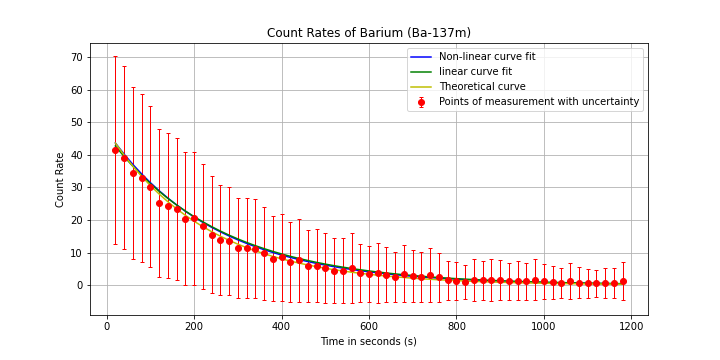
\includegraphics[width=0.95\linewidth]{../Exercise2/Fredrik/Count Rates of Barium (Ba-137m).png}    
  \begin{center}
    \emph{
      Relationship between count rates and time. We have plotted the points of measurement 
      with corresponding error bars, the curve of theoretical emission rate, and the two models 
      of emission rate best fitted to our data.}
  \end{center}
  \caption{Count Rates of Barium (Ba137-m)}
  \label{ba-count-rates}
\end{figure}

\begin{figure}[H]
  \centering
  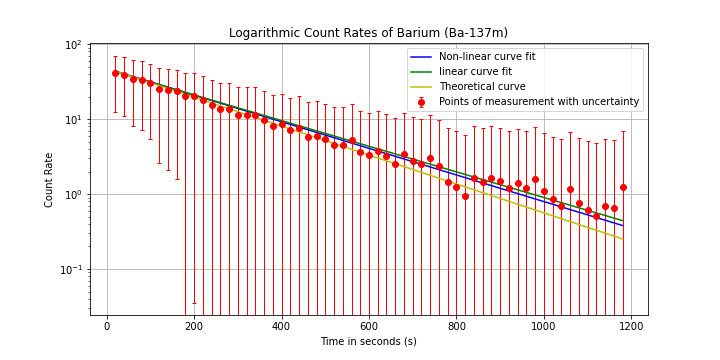
\includegraphics[width=0.95\linewidth]{../Exercise2/Fredrik/Logarithmic Count Rates of Barium (Ba-137m).png}   
  \begin{center}
    \emph{
      Equal to Figure 1, though with a logarithmic y-axis}
  \end{center}
  \caption{Logarithmic Count Rates of Barium (Ba137-m)}
  \label{ba-count-rates-log}
\end{figure}

\pagebreak

\subsection{Plots For Exercise 5}

\begin{figure}[H]
  \centering
  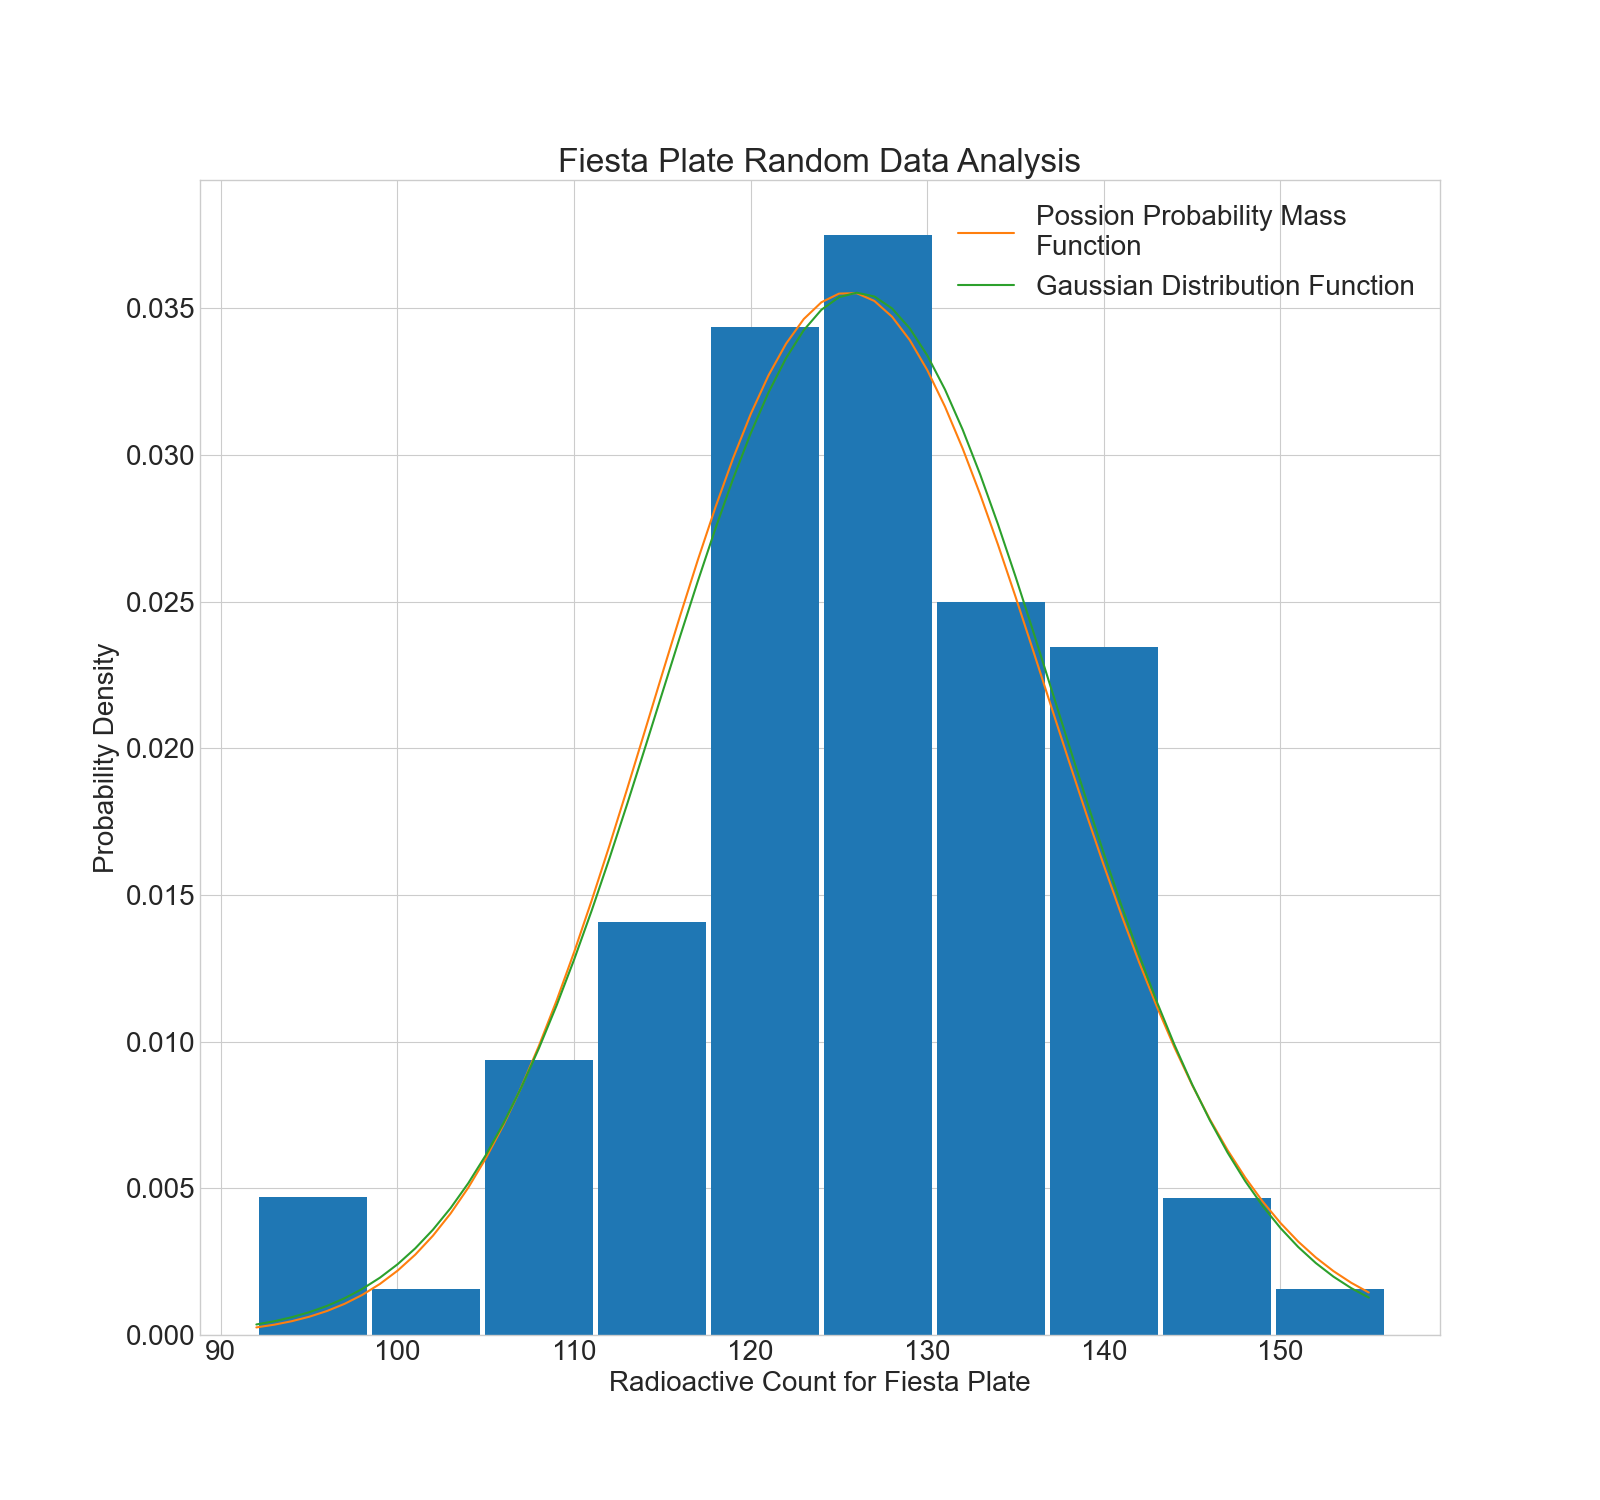
\includegraphics[width=0.95\linewidth]{../Exercise5/Pankaj/Fiesta Plate.png}    
  \caption{Random Data Analysis For Fiesta Plate Radioactive Counts}
  \label{fiesta-plate}
\end{figure}

\begin{figure}[H]
  \centering
  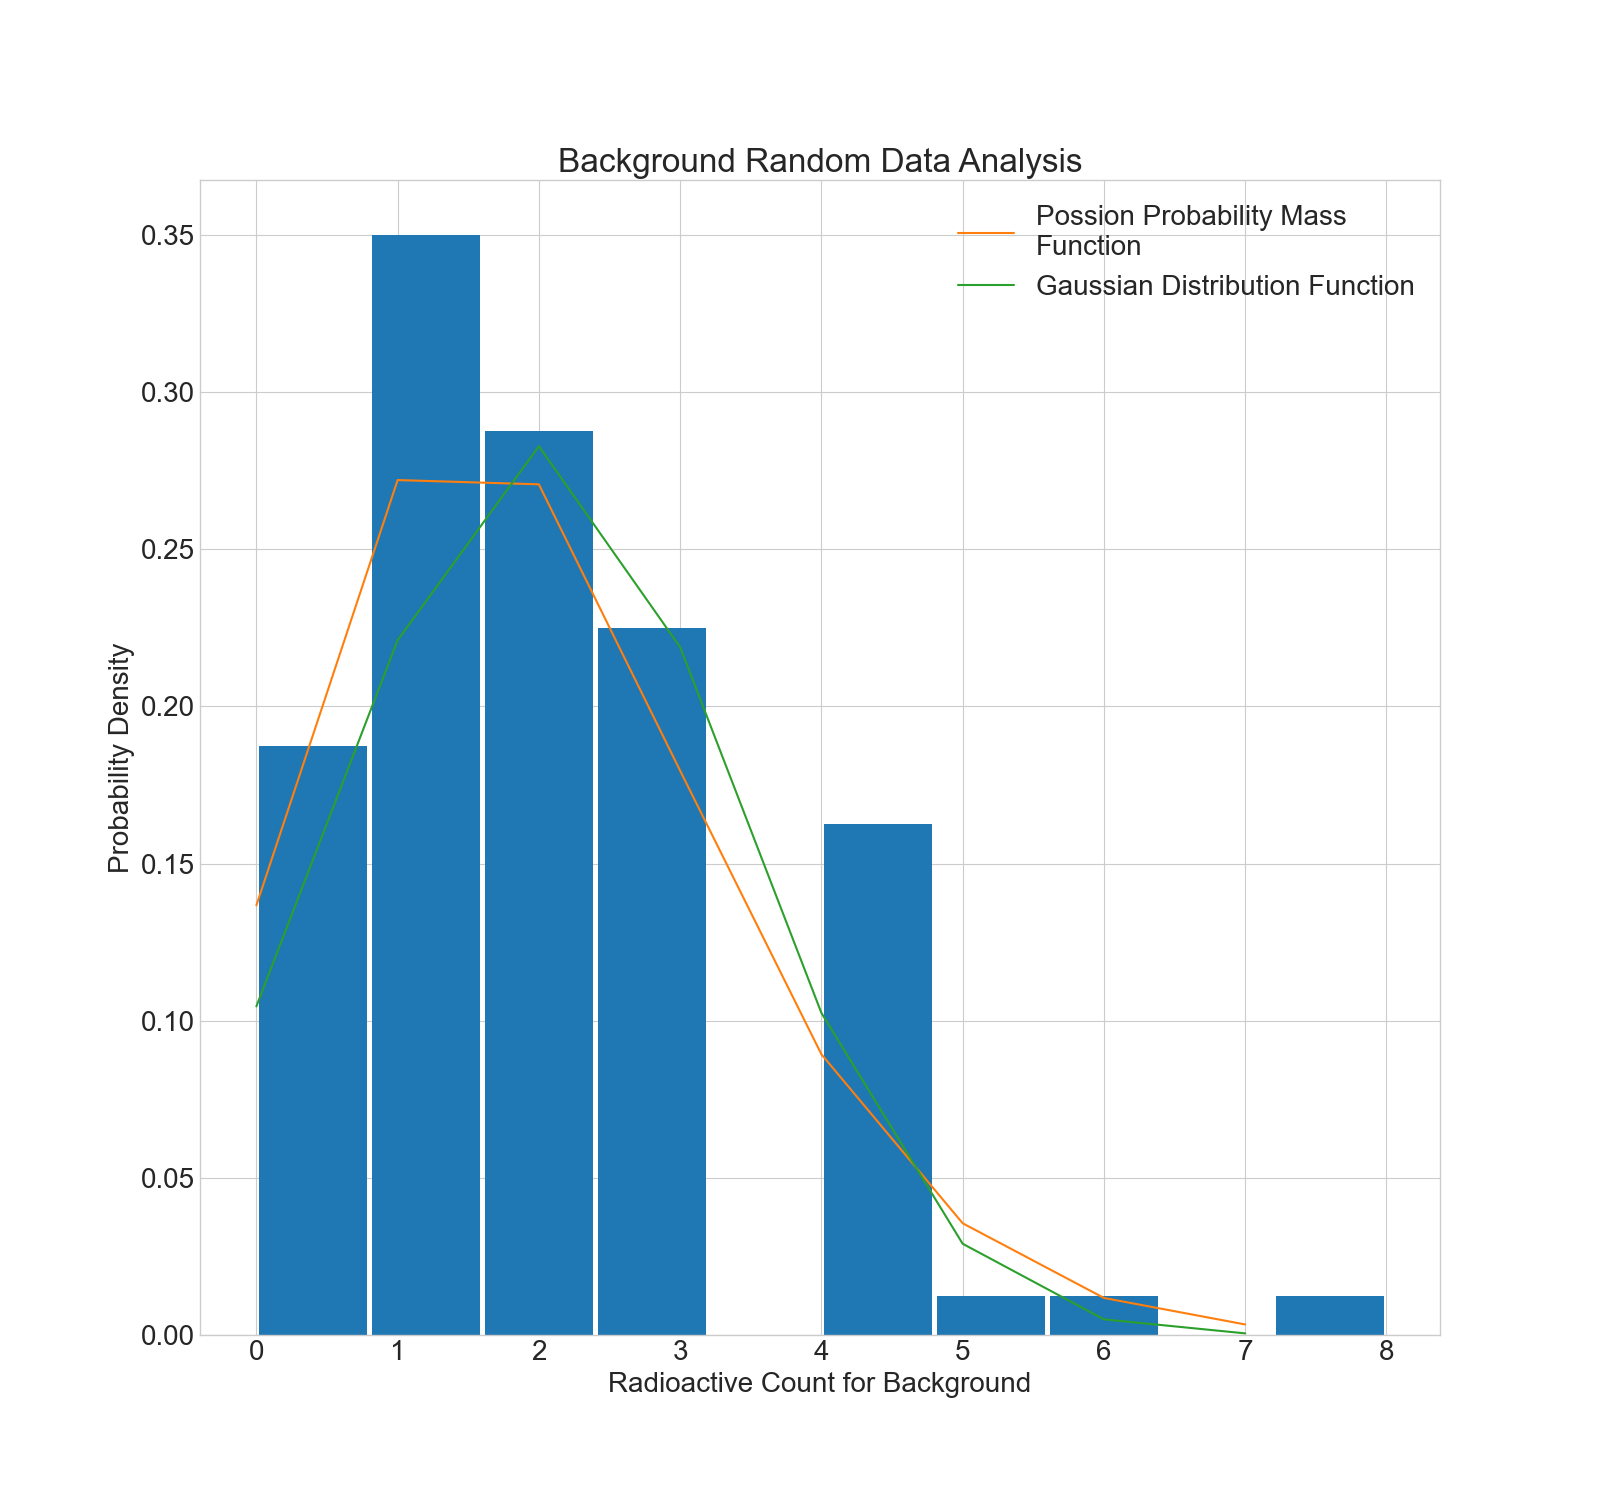
\includegraphics[width=0.95\linewidth]{../Exercise5/Pankaj/Background.png}    
  \caption{Random Data Analysis For Background Counts}
  \label{background}
\end{figure}

\pagebreak

\subsection{Python Code: Exercise 1}

The Python code for this exercise is divided into two files. Functions.py file contains utility methods
which we will be frequently using in this course. Radioactive Decay.py file contains the code which analyzes
the data.

\subsubsection{Functions.py}
\noindent\rule{\textwidth}{1pt}
\verbatiminput{../Exercise2/Fredrik/Functions.py}
\noindent\rule{\textwidth}{1pt}

\pagebreak

\subsubsection{Radioactive Decay.py}
\noindent\rule{\textwidth}{1pt}
\verbatiminput{../Exercise2/Fredrik/Radioactive Decay.py}
\noindent\rule{\textwidth}{1pt}

\pagebreak

\subsection{Python Code: Exercise 5}

The Python code for this exercise is divided into two files. statslab.py file 
contains utility methods
which we will be frequently using in this course. lab\_2\_ex\_5\_code.py file contains 
the code which analyzes
the data for this experiment.

\subsubsection{statslab.py}

\noindent\rule{\textwidth}{1pt}
\verbatiminput{../Exercise5/Pankaj/statslab.py}
\noindent\rule{\textwidth}{1pt}

\pagebreak

\subsubsection{lab\_2\_ex\_5\_code.py}
\noindent\rule{\textwidth}{1pt}
\verbatiminput{../Exercise5/Pankaj/lab_2_ex_5_code.py}
\noindent\rule{\textwidth}{1pt}
\pagebreak

\begin{thebibliography}{99}

\bibitem{lab-manual-ex2} Lab Manual - Nonlinear fitting methods I - Exercise 2.
\bibitem{lab-manual-ex5} Lab Manual - Random number analysis - Exercise 5.

\end{thebibliography}

\end{document}
